\documentclass[12pt, a4paper]{article}

% ── Packages ──────────────────────────────────────────────────────────────────
\usepackage[utf8]{inputenc}
\usepackage[T1]{fontenc}
\usepackage{lmodern}
\usepackage[margin=1in]{geometry}
\usepackage{graphicx}
\usepackage{amsmath, amssymb}
\usepackage{booktabs}
\usepackage{hyperref}
\usepackage{listings}
\usepackage{xcolor}
\usepackage{enumitem}
\usepackage{float}
\usepackage{caption}
\usepackage{parskip}
\usepackage{tikz}
\usetikzlibrary{positioning}
\usepackage{fancyhdr}

% ── Code listing style ───────────────────────────────────────────────────────
\definecolor{codebg}{RGB}{245,245,245}
\definecolor{codegreen}{RGB}{0,128,0}
\definecolor{codegray}{RGB}{128,128,128}
\definecolor{codepurple}{RGB}{128,0,128}

\lstdefinestyle{pythonstyle}{
    backgroundcolor=\color{codebg},
    basicstyle=\ttfamily\small,
    breaklines=true,
    captionpos=b,
    commentstyle=\color{codegreen},
    keywordstyle=\color{blue}\bfseries,
    stringstyle=\color{codepurple},
    numberstyle=\tiny\color{codegray},
    numbers=left,
    numbersep=8pt,
    frame=single,
    rulecolor=\color{gray!40},
    language=Python,
    showstringspaces=false,
    tabsize=4,
    morekeywords={self, True, False, None, as, with, lambda},
}
\lstset{style=pythonstyle}

% ── Header / Footer ──────────────────────────────────────────────────────────
\pagestyle{fancy}
\fancyhf{}
\rhead{Music Listening Behaviour — Time Series Analysis}
\lhead{ML Project Report}
\cfoot{\thepage}

% ── Title ─────────────────────────────────────────────────────────────────────
\title{
    \vspace{-1cm}
    \textbf{Predicting Music Listening Behaviour\\Using Time Series Analysis}\\[0.5em]
    \large A Beginner-Friendly Guide to the Complete Pipeline:\\
    Feature Engineering $\rightarrow$ Daily Aggregation $\rightarrow$ SARIMA Forecasting
}
\author{ML Project Team}
\date{\today}

% ══════════════════════════════════════════════════════════════════════════════
\begin{document}
\maketitle
\thispagestyle{fancy}

\begin{abstract}
This report explains, step by step, a machine-learning project that analyses
real-world music listening data from \textbf{Last.fm}. The goal is to
understand \emph{when} people listen to music by aggregating raw scrobble
logs into daily play-count time series, and then \textbf{forecast future
daily play counts} using a SARIMA model. The approach is deliberately simple
--- no embeddings, no SVD, no clustering --- just counting plays per day and
modelling that count over time. Every concept is introduced from scratch so
that a beginner can follow along, reproduce the results, and present them
confidently.
\end{abstract}

\tableofcontents
\newpage

% ══════════════════════════════════════════════════════════════════════════════
\section{Introduction}
% ══════════════════════════════════════════════════════════════════════════════

\subsection{What Is This Project About?}
Imagine you have a record of every song a group of people played over the
course of a month. This project takes that record and asks two key questions:

\begin{enumerate}
    \item \textbf{When do people listen?} — Do they listen more in the
          morning or at night? On weekdays or weekends? Are there weekly
          patterns?
    \item \textbf{Can we predict future listening?} — Given past daily play
          counts, can we forecast how many songs a user will play tomorrow or
          next week?
\end{enumerate}

The approach is intentionally straightforward: aggregate raw listening events
into a \textbf{daily play-count time series} for a single user, then apply
classical time series techniques (stationarity testing, seasonal
decomposition, ACF/PACF analysis) to fit a \textbf{SARIMA model} that
forecasts future activity.

\subsection{Why Does This Matter?}
Music streaming platforms (Spotify, Apple Music, YouTube Music) use exactly
these techniques to:
\begin{itemize}
    \item Schedule push notifications at the right time of day.
    \item Predict server load for capacity planning.
    \item Understand user engagement trends over time.
    \item Detect changes in listening behaviour (e.g.\ a user becoming less
          active).
\end{itemize}

% ══════════════════════════════════════════════════════════════════════════════
\section{The Dataset}
% ══════════════════════════════════════════════════════════════════════════════

\subsection{Source}
The data comes from \textbf{Last.fm}, a music tracking service that logs
every song (called a \emph{scrobble}) a user plays. The dataset is stored in
\texttt{fm\_data.csv}.

\subsection{Size and Shape}
\begin{center}
\begin{tabular}{ll}
    \toprule
    \textbf{Property} & \textbf{Value} \\
    \midrule
    Total rows (scrobbles)   & 166{,}153  \\
    Number of users          & 11         \\
    Unique artists           & 22{,}823   \\
    Unique tracks            & 67{,}241   \\
    Date range               & 1 Jan 2021 -- 31 Jan 2021 (31 days) \\
    \bottomrule
\end{tabular}
\end{center}

\subsection{Columns}

\begin{center}
\begin{tabular}{lp{9cm}}
    \toprule
    \textbf{Column} & \textbf{Description} \\
    \midrule
    \texttt{Username} & The Last.fm username (e.g.\ \texttt{Babs\_05}). \\
    \texttt{Artist}   & The artist name. \\
    \texttt{Track}    & The track (song) name. \\
    \texttt{Album}    & The album the track belongs to. \\
    \texttt{Date}     & The calendar date (e.g.\ \texttt{31 Jan 2021}). \\
    \texttt{Time}     & The clock time (e.g.\ \texttt{23:36}). \\
    \bottomrule
\end{tabular}
\end{center}

\subsection{Per-User Play Counts}
Not all users are equally active. Here is how the scrobbles are distributed:

\begin{center}
\begin{tabular}{lr}
    \toprule
    \textbf{Username} & \textbf{Play Count} \\
    \midrule
    Babs\_05     & 33{,}695 \\
    franhale     & 32{,}712 \\
    Knapster01   & 27{,}015 \\
    eartle       & 20{,}966 \\
    massdosage   & 19{,}015 \\
    jonocole     & 17{,}230 \\
    Orlenay      & 10{,}123 \\
    isaac        & 1{,}780  \\
    mremond      & 1{,}452  \\
    jajo         & 1{,}102  \\
    lobsterclaw  & 1{,}063  \\
    \bottomrule
\end{tabular}
\end{center}

\subsection{A Peek at the Raw Data}
Each row records one listening event:

\begin{center}
\small
\begin{tabular}{llllll}
    \toprule
    \textbf{Username} & \textbf{Artist} & \textbf{Track} & \textbf{Album} & \textbf{Date} & \textbf{Time} \\
    \midrule
    Babs\_05 & Isobel Campbell & The Circus Is\ldots & Ballad of\ldots & 31 Jan 2021 & 23:36 \\
    Babs\_05 & Isobel Campbell & Dusty Wreath       & Ballad of\ldots & 31 Jan 2021 & 23:32 \\
    Babs\_05 & The Coral       & Sandhills\ldots     & Lockdown\ldots  & 31 Jan 2021 & 22:56 \\
    \bottomrule
\end{tabular}
\end{center}

% ══════════════════════════════════════════════════════════════════════════════
\section{High-Level Pipeline Overview}
% ══════════════════════════════════════════════════════════════════════════════

The entire project flows through five major stages. Each stage feeds into the
next:

\begin{center}
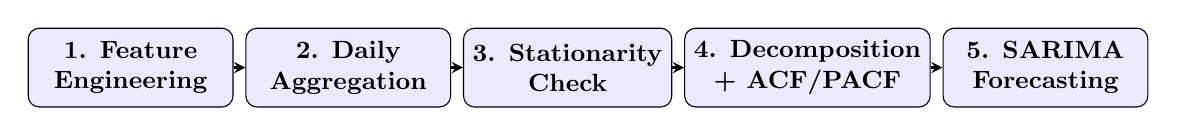
\begin{tikzpicture}[
    node distance=0.15cm and 0.15cm,
    box/.style={draw, rounded corners, minimum width=2.6cm, minimum height=1cm,
                align=center, font=\small\bfseries, fill=blue!8},
    arrow/.style={->, thick, >=stealth}
]
    \node[box] (fe)   {1. Feature\\Engineering};
    \node[box, right=of fe]  (agg)  {2. Daily\\Aggregation};
    \node[box, right=of agg] (stat) {3. Stationarity\\Check};
    \node[box, right=of stat](dec)  {4. Decomposition\\+ ACF/PACF};
    \node[box, right=of dec] (ts)   {5. SARIMA\\Forecasting};
    \draw[arrow] (fe)   -- (agg);
    \draw[arrow] (agg)  -- (stat);
    \draw[arrow] (stat) -- (dec);
    \draw[arrow] (dec)  -- (ts);
\end{tikzpicture}
\end{center}

\begin{enumerate}
    \item \textbf{Feature Engineering} — Parse dates/times, create new
          columns (hour, day of week, time period, weekend flag).
    \item \textbf{Daily Aggregation} — For a chosen user, count the number
          of plays per day to produce a daily time series.
    \item \textbf{Stationarity Check} — Use the Augmented Dickey--Fuller
          (ADF) test to determine whether the series is stationary; apply
          differencing if it is not.
    \item \textbf{Decomposition + ACF/PACF} — Decompose the series into
          trend, seasonality, and residual; inspect ACF and PACF plots to
          guide model order selection.
    \item \textbf{SARIMA Forecasting} — Fit a Seasonal ARIMA model on 80\%
          of the data and forecast the remaining 20\%, evaluating with MAE.
\end{enumerate}

% ══════════════════════════════════════════════════════════════════════════════
\section{Step 1 — Feature Engineering}
% ══════════════════════════════════════════════════════════════════════════════

\subsection{What Is Feature Engineering?}
Raw data rarely comes in a form that machine-learning models can use directly.
\textbf{Feature engineering} is the process of transforming raw columns into
new, more informative columns (called \emph{features}).

\subsection{Combining Date and Time}
The CSV stores the date and time in separate text columns. We merge them into
a single \texttt{datetime} object so that Python can do arithmetic on it
(e.g.\ compute differences, extract parts):

\begin{lstlisting}
df['datetime'] = pd.to_datetime(
    df['Date'] + ' ' + df['Time'], dayfirst=True
)
df = df.sort_values('datetime').reset_index(drop=True)
\end{lstlisting}

\texttt{dayfirst=True} tells pandas that the day comes before the month
(\texttt{31 Jan 2021}, not \texttt{Jan 31 2021}).

\subsection{Extracting the Hour}
From the datetime we pull out the \textbf{hour} (0--23):

\begin{lstlisting}
df['hour'] = df['datetime'].dt.hour
\end{lstlisting}

This single number tells us \emph{when} during the day a song was played.

\subsection{Time Period Bins}
Hours are fine-grained. For a simpler picture we group them into four
\textbf{time periods}:

\begin{center}
\begin{tabular}{lc}
    \toprule
    \textbf{Period} & \textbf{Hours} \\
    \midrule
    Morning   & 05:00 -- 11:59 \\
    Afternoon & 12:00 -- 16:59 \\
    Evening   & 17:00 -- 20:59 \\
    Night     & 21:00 -- 04:59 \\
    \bottomrule
\end{tabular}
\end{center}

\begin{lstlisting}
def time_period(hour):
    if   5 <= hour < 12: return 'Morning'
    elif 12 <= hour < 17: return 'Afternoon'
    elif 17 <= hour < 21: return 'Evening'
    else:                 return 'Night'

df['period'] = df['hour'].apply(time_period)
\end{lstlisting}

\subsection{Day of the Week and Weekend Flag}
\begin{lstlisting}
df['day_of_week'] = df['datetime'].dt.day_name()
df['is_weekend']  = df['day_of_week'].isin(['Saturday', 'Sunday'])
\end{lstlisting}

\textbf{Why?} Listening habits often differ between weekdays and weekends.
Someone might listen to focus music on Monday and party music on Saturday.

\subsection{Summary of Engineered Features}

\begin{center}
\begin{tabular}{llp{7cm}}
    \toprule
    \textbf{Feature} & \textbf{Type} & \textbf{Purpose} \\
    \midrule
    \texttt{datetime}     & Timestamp    & Single sortable time column. \\
    \texttt{hour}         & Integer 0--23 & Fine-grained time of day. \\
    \texttt{period}       & Categorical  & Coarse time of day (Morning, etc.). \\
    \texttt{day\_of\_week}& Categorical  & Which day (Monday\ldots Sunday). \\
    \texttt{is\_weekend}  & Boolean      & Weekday vs.\ weekend. \\
    \texttt{date\_only}   & Date         & Calendar date for daily aggregation. \\
    \bottomrule
\end{tabular}
\end{center}

% ══════════════════════════════════════════════════════════════════════════════
\section{Step 2 --- Aggregating to a Daily Time Series}
% ══════════════════════════════════════════════════════════════════════════════

\subsection{Why Aggregate?}
The raw data contains one row per scrobble (166{,}153 rows). To perform time
series analysis we need a single number per time step. The simplest and most
natural choice is to \textbf{count the number of plays per day} for one user.

\subsection{Choosing a User}
We start with the most active user, \texttt{Babs\_05} (33{,}695 scrobbles),
because a higher play count gives the time series more variation and makes
patterns easier to detect.

\subsection{Code}

\begin{lstlisting}
user = 'Babs_05'
user_df = df[df['Username'] == user]

# Count plays per day
ts = user_df.groupby(user_df['datetime'].dt.date).size()
ts.index = pd.to_datetime(ts.index)
ts = ts.asfreq('D').fillna(0)  # fill days with no listens as 0
\end{lstlisting}

\subsection{What Each Line Does}

\begin{enumerate}
    \item \textbf{Filter} the dataframe to keep only rows belonging to
          \texttt{Babs\_05}.
    \item \textbf{Group by date} and count the number of rows (scrobbles)
          per day using \texttt{.size()}.
    \item \textbf{Convert the index} to proper \texttt{DatetimeIndex} so
          that pandas recognises it as a time series.
    \item \textbf{\texttt{asfreq('D')}} ensures every calendar day is
          present in the index --- even days on which the user did not listen.
          Without this step, missing days would create gaps that confuse
          time series models.
    \item \textbf{\texttt{fillna(0)}} fills those newly created gaps with
          zero, meaning ``no plays that day''.
\end{enumerate}

The result is a \texttt{pandas.Series} of length 31 (one value per day in
January 2021) with integer play counts.

% ══════════════════════════════════════════════════════════════════════════════
\section{Step 3 --- Stationarity, Decomposition, and ACF/PACF}
% ══════════════════════════════════════════════════════════════════════════════

This step prepares the daily time series for modelling by checking its
statistical properties and analysing its structure.

\subsection{What Is a Time Series?}
A time series is any sequence of data points indexed by time:
\[
    y_1, \; y_2, \; y_3, \; \ldots, \; y_T
\]
In our case $y_t$ = number of songs played on day $t$. With 31 days of data
we have $T = 31$.

\subsection{Stationarity and the ADF Test}

\subsubsection{What Is Stationarity?}
A time series is \textbf{stationary} if its statistical properties (mean,
variance) do not change over time. Most forecasting models require (or work
best with) stationary data.

\subsubsection{Augmented Dickey--Fuller (ADF) Test}
The ADF test is a statistical hypothesis test:
\begin{itemize}
    \item \textbf{Null hypothesis $H_0$}: The series has a unit root (it is
          \emph{non-stationary}).
    \item \textbf{Alternative $H_1$}: The series is stationary.
\end{itemize}
If the \textbf{p-value $< 0.05$} we reject $H_0$ and conclude the series is
stationary.

\begin{lstlisting}
from statsmodels.tsa.stattools import adfuller

result = adfuller(ts)
print(f'p-value: {result[1]:.4f}')
# p < 0.05  ->  stationary (good to go)
# p >= 0.05 ->  difference the series
\end{lstlisting}

\subsubsection{Differencing}
If the series is non-stationary we apply \textbf{differencing}:
\[
    y'_t = y_t - y_{t-1}
\]
This removes trends. If one round is not enough, we difference again
(second-order differencing).

\subsection{Seasonal Decomposition}

Any time series can be decomposed into three components:
\[
    y_t = T_t + S_t + R_t
\]
\begin{itemize}
    \item $T_t$ — \textbf{Trend}: the long-term direction (increasing,
          decreasing, or flat).
    \item $S_t$ — \textbf{Seasonality}: repeating patterns at a fixed period
          (e.g.\ weekly).
    \item $R_t$ — \textbf{Residual}: the leftover noise.
\end{itemize}

\begin{lstlisting}
from statsmodels.tsa.seasonal import seasonal_decompose

result = seasonal_decompose(ts, model='additive', period=7)
result.plot()
\end{lstlisting}

We choose \texttt{period=7} because listening patterns are expected to repeat
weekly (e.g.\ less listening on workdays, more on weekends).

\subsection{ACF and PACF Plots}

\subsubsection{Autocorrelation Function (ACF)}
The ACF measures the correlation between $y_t$ and $y_{t-k}$ for various
lags $k$. It answers: ``How much does today's value depend on past values?''

\subsubsection{Partial Autocorrelation Function (PACF)}
The PACF measures the correlation between $y_t$ and $y_{t-k}$ \emph{after
removing the effects of all intermediate lags}. It helps isolate the
\emph{direct} influence of lag $k$.

\begin{lstlisting}
from statsmodels.graphics.tsaplots import plot_acf, plot_pacf

plot_acf(ts, lags=30)
plot_pacf(ts, lags=30)
\end{lstlisting}

\subsubsection{How to Read ACF/PACF}
\begin{center}
\begin{tabular}{lcc}
    \toprule
    \textbf{Pattern} & \textbf{ACF} & \textbf{PACF} \\
    \midrule
    AR($p$) process  & Tails off gradually & Cuts off after lag $p$ \\
    MA($q$) process  & Cuts off after lag $q$ & Tails off gradually \\
    ARMA($p,q$)      & Tails off & Tails off \\
    \bottomrule
\end{tabular}
\end{center}

These patterns guide the choice of model orders (see SARIMA below).

\subsection{SARIMA Model}

\subsubsection{What Is ARIMA?}
ARIMA stands for \textbf{A}uto\textbf{R}egressive \textbf{I}ntegrated
\textbf{M}oving \textbf{A}verage. It has three parts controlled by the order
$(p, d, q)$:

\begin{itemize}
    \item $p$ (\textbf{AR} — Auto-Regressive): Number of past values used as
          predictors.
          \[
              y_t = c + \phi_1 y_{t-1} + \phi_2 y_{t-2} + \cdots +
              \phi_p y_{t-p} + \epsilon_t
          \]
    \item $d$ (\textbf{I} — Integrated): Number of times the series is
          differenced to make it stationary.
    \item $q$ (\textbf{MA} — Moving Average): Number of past forecast errors
          used as predictors.
          \[
              y_t = c + \epsilon_t + \theta_1 \epsilon_{t-1} + \cdots +
              \theta_q \epsilon_{t-q}
          \]
\end{itemize}

\subsubsection{Adding Seasonality: SARIMA}
SARIMA extends ARIMA with a seasonal component. Its full specification is:
\[
    \text{SARIMA}(p, d, q) \times (P, D, Q, s)
\]
where $(P, D, Q)$ are the seasonal AR, differencing, and MA orders, and $s$
is the seasonal period (7 for weekly).

\begin{lstlisting}
from statsmodels.tsa.statespace.sarimax import SARIMAX

model = SARIMAX(ts, order=(1,0,1),
                seasonal_order=(1,0,1,7))
result = model.fit()
print(result.summary())
\end{lstlisting}

In our case:
\begin{itemize}
    \item $(p,d,q) = (1,0,1)$: one AR lag, no differencing, one MA lag.
    \item $(P,D,Q,s) = (1,0,1,7)$: one seasonal AR lag, no seasonal differencing,
          one seasonal MA lag, weekly seasonality.
\end{itemize}

% ══════════════════════════════════════════════════════════════════════════════
\section{Step 4 --- SARIMA Forecasting and Evaluation}
% ══════════════════════════════════════════════════════════════════════════════

This section covers the core modelling step: fitting a SARIMA model on a
training portion of the daily time series and evaluating its forecast on a
held-out test set.

\subsection{Train/Test Split (Temporal)}
For time series data we \textbf{never shuffle}. We split chronologically:

\begin{lstlisting}
split = int(len(ts) * 0.8)
train, test = ts[:split], ts[split:]
\end{lstlisting}

The first 80\% of days are used for training; the last 20\% for testing.
This prevents \textbf{data leakage} — using future data to predict the past.

\subsection{Evaluation Metric: MAE}

\textbf{Mean Absolute Error} measures average prediction error in the same
units as the data (plays per day):
\[
    \text{MAE} = \frac{1}{n} \sum_{i=1}^{n} |y_i - \hat{y}_i|
\]

\begin{lstlisting}
from sklearn.metrics import mean_absolute_error
print(f'MAE: {mean_absolute_error(y_test, y_pred):.2f}')
\end{lstlisting}

A lower MAE means better predictions.

\subsection{Forecasting and Plotting}
The final step is to generate predictions on the test set and visualise them:

\begin{lstlisting}
model = SARIMAX(train, order=(1,0,1),
                seasonal_order=(1,0,1,7)).fit()
forecast = model.forecast(steps=len(test))

pd.DataFrame({'actual': test, 'forecast': forecast}).plot()
\end{lstlisting}

This produces a plot with:
\begin{itemize}
    \item The \textbf{training data} (historical context).
    \item The \textbf{actual} test values (ground truth).
    \item The \textbf{forecast} line (model predictions).
\end{itemize}

% ══════════════════════════════════════════════════════════════════════════════
\section{Concepts Glossary}
% ══════════════════════════════════════════════════════════════════════════════

For quick reference, here is every key concept used in this project:

\begin{center}
\small
\begin{tabular}{p{4cm}p{10cm}}
    \toprule
    \textbf{Concept} & \textbf{One-Line Explanation} \\
    \midrule
    Feature Engineering    & Creating new informative columns from raw data. \\
    Time Series            & A sequence of data points indexed in time order. \\
    Stationarity           & Statistical properties (mean, variance) constant over time. \\
    ADF Test               & Statistical test for stationarity (Augmented Dickey--Fuller). \\
    Differencing           & Subtracting consecutive values to remove trends: $y'_t = y_t - y_{t-1}$. \\
    Seasonal Decomposition & Splitting a series into trend, seasonality, and residual. \\
    ACF                    & Autocorrelation function --- correlation of a series with its own lagged values. \\
    PACF                   & Partial autocorrelation --- direct correlation at lag $k$, removing intermediate effects. \\
    AR (Auto-Regressive)   & Using past values of the series as predictors. \\
    MA (Moving Average)    & Using past forecast errors as predictors. \\
    ARIMA                  & Model combining AR, differencing, and MA components. \\
    SARIMA                 & ARIMA extended with seasonal AR, differencing, and MA terms. \\
    MAE                    & Mean Absolute Error --- average prediction error magnitude. \\
    Train/Test Split       & Dividing data chronologically to evaluate model performance. \\
    Data Leakage           & Accidentally using future information during training. \\
    \texttt{asfreq('D')}   & Ensures every calendar day appears in the index (fills gaps). \\
    \texttt{fillna(0)}     & Replaces missing values with zero (no plays that day). \\
    \bottomrule
\end{tabular}
\end{center}

% ══════════════════════════════════════════════════════════════════════════════
\section{Libraries and Tools Used}
% ══════════════════════════════════════════════════════════════════════════════

\begin{center}
\begin{tabular}{llp{7.5cm}}
    \toprule
    \textbf{Library} & \textbf{Version} & \textbf{Role in This Project} \\
    \midrule
    pandas          & 3.0.1  & Data loading, manipulation, grouping, time series indexing (\texttt{asfreq}, \texttt{fillna}). \\
    NumPy           & 2.4.2  & Numerical operations on arrays. \\
    scikit-learn    & 1.8.0  & \texttt{mean\_absolute\_error} for evaluation. \\
    statsmodels     & ---    & ADF test, seasonal decomposition, ACF/PACF plotting, SARIMAX model. \\
    matplotlib      & 3.10.8 & All plots and charts. \\
    \bottomrule
\end{tabular}
\end{center}

% ══════════════════════════════════════════════════════════════════════════════
\section{Project File Structure}
% ══════════════════════════════════════════════════════════════════════════════

\begin{center}
\begin{tabular}{lp{9cm}}
    \toprule
    \textbf{File / Folder} & \textbf{Description} \\
    \midrule
    \texttt{fm\_data.csv}                    & Raw Last.fm scrobble data (166{,}153 rows). \\
    \texttt{info.txt}                        & Step-by-step plan for the time series analysis pipeline. \\
    \texttt{requirements.txt}                & Python dependencies with pinned versions. \\
    \texttt{project\_report.tex}             & This report (LaTeX source). \\
    \texttt{time\_feature\_engineering.ipynb} & Notebook for feature engineering exploration. \\
    \texttt{test.ipynb}                      & Notebook: time series analysis and SARIMA forecasting. \\
    \texttt{test2.ipynb}                     & Notebook: additional forecasting experiments. \\
    \bottomrule
\end{tabular}
\end{center}

% ══════════════════════════════════════════════════════════════════════════════
\section{Putting It All Together — End-to-End Walkthrough}
% ══════════════════════════════════════════════════════════════════════════════

\begin{enumerate}[leftmargin=*, label=\textbf{Step \arabic*}.]
    \item \textbf{Load the CSV} and parse \texttt{Date + Time} into a
          single \texttt{datetime} column.
    \item \textbf{Engineer features}: extract hour, time period, day of week,
          and weekend flag for exploratory analysis.
    \item \textbf{Pick a user} (e.g.\ \texttt{Babs\_05}) and \textbf{count
          plays per day} to create a daily time series.
    \item \textbf{Fill gaps}: use \texttt{asfreq('D').fillna(0)} so every
          calendar day has a value.
    \item \textbf{Check stationarity} with the ADF test; difference the
          series if the p-value $\geq 0.05$.
    \item \textbf{Decompose} into trend, seasonality (period = 7), and
          residual.
    \item \textbf{Inspect ACF/PACF} plots to determine appropriate SARIMA
          orders $(p, d, q)$ and $(P, D, Q, s)$.
    \item \textbf{Split chronologically}: first 80\% for training, last
          20\% for testing.
    \item \textbf{Fit a SARIMA model} on the training set with
          \texttt{SARIMAX(train, order=(1,0,1),
          seasonal\_order=(1,0,1,7))}.
    \item \textbf{Forecast} the test period and compute MAE.
    \item \textbf{Plot actual vs.\ forecast} to visually assess model
          quality.
\end{enumerate}

% ══════════════════════════════════════════════════════════════════════════════
\section{Potential Improvements}
% ══════════════════════════════════════════════════════════════════════════════

\begin{itemize}
    \item \textbf{More data}: One month (31 days) is short. With several
          months the model could learn longer-term seasonal and monthly
          patterns more reliably.
    \item \textbf{Auto-ARIMA}: Use \texttt{pmdarima.auto\_arima} to
          automatically search for the best $(p,d,q)(P,D,Q,s)$ orders
          instead of manually reading ACF/PACF plots.
    \item \textbf{Prophet / Neural models}: Facebook Prophet or LSTM networks
          can capture complex non-linear patterns.
    \item \textbf{Multi-user modelling}: Instead of one user at a time, model
          all users jointly or compare SARIMA fits across users.
    \item \textbf{Exogenous variables}: Feed day-of-week, time-period
          proportions, or external data (e.g.\ weather, holidays) as
          regressors into SARIMAX.
    \item \textbf{Cross-validation}: Use rolling-window or expanding-window
          cross-validation instead of a single 80/20 split for more robust
          evaluation.
\end{itemize}

% ══════════════════════════════════════════════════════════════════════════════
\section{Conclusion}
% ══════════════════════════════════════════════════════════════════════════════

This project demonstrates a complete, beginner-friendly time series analysis
pipeline on real music listening data:

\begin{enumerate}
    \item We \textbf{engineered features} from raw timestamps to understand
          listening patterns by hour, time period, and day of week.
    \item We \textbf{aggregated} raw scrobble events into a \textbf{daily
          play-count time series} for a single user.
    \item We checked \textbf{stationarity} using the ADF test and
          \textbf{decomposed} the series into trend, seasonality, and
          residual components.
    \item We used \textbf{ACF and PACF} plots to guide the selection of
          model orders.
    \item We fit a \textbf{SARIMA model} on the training data and
          \textbf{forecast} future daily play counts, evaluating accuracy
          with MAE.
\end{enumerate}

The pipeline is deliberately simple --- no embeddings, no dimensionality
reduction, no clustering --- just counting plays and modelling that count
over time. This makes every step easy to understand, reproduce, and extend.

% ══════════════════════════════════════════════════════════════════════════════
\end{document}
